\documentclass[12pt,addpoints]{repaso}
\grado{5}
\nivel{Primaria}
\cicloescolar{2024-2025}
\materia{Matemáticas}
\unidad{3}
\title{Practica la Unidad}
\aprendizajes{\scriptsize%
	% \item Estudio de los números.
\item Ordena, lee, escribe e identifica regularidades en números naturales de hasta nueve cifras. Lee, escribe y ordena números decimales hasta diezmilésimos en notación decimal y letra, y los interpreta en diferentes contextos.
	% \item Suma y resta, su relación como operaciones inversas.
	\item Propone y resuelve situaciones problemáticas que implican sumas y restas con números decimales utilizando el algoritmo convencional y fracciones con diferentes denominadores. 
	% \item Multiplicación y división, su relación como operaciones inversas.
	\item Resuelve situaciones problemáticas vinculadas a diferentes contextos que implican multiplicar números fraccionarios y números decimales, con un número natural como multiplicador.También, dividir números naturales y el cociente resulte un número decimal.
	% \item Relaciones de proporcionalidad.
	\item Resuelve situaciones problemáticas de proporcionalidad en las que determina valores faltantes de números naturales, a partir de diferentes estrategias (cálculo del valor unitario, de dobles, triples o mitades).
	% \item Ubicación espacial.
	\item Elabora e interpreta croquis para comunicar la ubicación de seres vivos, objetos, trayectos o lugares.
	% \item Medición de la longitud, masa y capacidad.
	% \item Figuras y cuerpos geométricos y sus características.
	\item Reconoce y describe semejanzas y diferencias entre un prisma y una pirámide; propone desarrollos planos para construir prismas rectos cuadrangulares o rectangulares.
	% \item Perímetro, área y noción de volumen.
	\item Calcula el perímetro y área de diferentes polígonos. Construye y usa fórmulas para calcular el perímetro de cualquier polígono, a partir de sumar la longitud de todos sus lados o multiplicar el número de lados por la medida de uno de ellos.
	% \item Organización e interpretación de datos.
	\item Construye tablas y gráficas de barras, e interpreta información cuantitativa y cualitativa contenida en ellas.
	% \item Nociones de probabilidad. 
	\item Identifica situaciones de distintos contextos en las que interviene o no el azar; registra resultados de experiencias aleatorias en tablas de frecuencias y expresa la frecuencia absoluta y la relativa.
	  }
\author{Melchor Pinto, JC}
\begin{document}
\INFO
\begin{multicols}{2}
	\tableofcontents
\end{multicols}
\begin{questions}\large
	\addcontentsline{toc}{section}{Unidad 3}
	\section*{Unidad 3}
	\addcontentsline{toc}{subsection}{Estadística y gráficas}
	\subsection*{Estadística y gráficas}
	% \subsection*{\ifprintanswers{Mediana    }                                            
	% \subsection*{\ifprintanswers{Moda       }                                            
	% \subsection*{\ifprintanswers{Media      }

	\questionboxed[2]{Determina la mediana y la moda en los siguientes conjuntos de datos:

		\begin{multicols}{2}
			\begin{parts}
				\part 80, 82, 85, 88, 90, 88, 91, 85, 95, 88, 88, 97, 100. \\[1em]
				La media es: \fillin[$89$][0.4in]. \\
				La mediana es: \fillin[$88$][0.4in].\\
				La moda es: \fillin[$88$][0.4in].  \\

				\part Los puntajes obtenidos en un juego son: 54, 55, 59, 61, 77, 58, 55, 71, 59, 55, 60, 53, 56 y 60 puntos. \\[1em]
				La media es: \fillin[$59.5$][0.4in]. \\
				La mediana es: \fillin[$58.5$][0.4in].\\
				La moda es: \fillin[$55$][0.4in]. \\
				% La desviación media es: \fillin[$4.5$][0.4in].

				\part 22, 25, 21, 23, 29, 30, 28, 27, 23, 26. \\[1em]
				La media es: \fillin[$25.4$][0.4in]. \\
				La mediana es: \fillin[$25.5$][0.4in].\\
				La moda es: \fillin[$23$][0.4in].\\
				% La desviación media es: \fillin[$2.6$][0.4in].

				\part Las estaturas de un grupo de personas son: 170, 168, 169, 171, 168, 172, 168, 171 y 173 cm. \\[1em]
				La media es: \fillin[$170$][0.4in]. \\
				La mediana es: \fillin[$170$][0.4in].\\
				La moda es: \fillin[$168$][0.4in]. \\
			\end{parts}
		\end{multicols}
	}

	% \subsection*{\ifprintanswers{Interpretación de gráficas         }
	\questionboxed[2]{Los resultados de una encuesta se muestran en la siguiente gráfica de barras:

		\begin{multicols}{2}
			\begin{parts}\normalsize
				\part ¿Cuántas personas participaron en la encuesta? \fillin[95][1.5cm]

				\part  ¿Cuál es la fruta menos preferida por las personas? \fillin[naranja][1.5cm]

				\part  ¿Cuál es la fruta preferida por las personas? \fillin[manzana][1.5cm]

				\part ¿Cuántas personas prefieren a las \textit{manzanas}.\fillin[29][1.5cm]

				\part ¿Cuántas personas prefieren a los \textit{plátanos}.\fillin[21][1.5cm]

				\part ¿Cuántas personas prefieren a las \textit{naranjas}.\fillin[19][1.5cm]

				\columnbreak%

				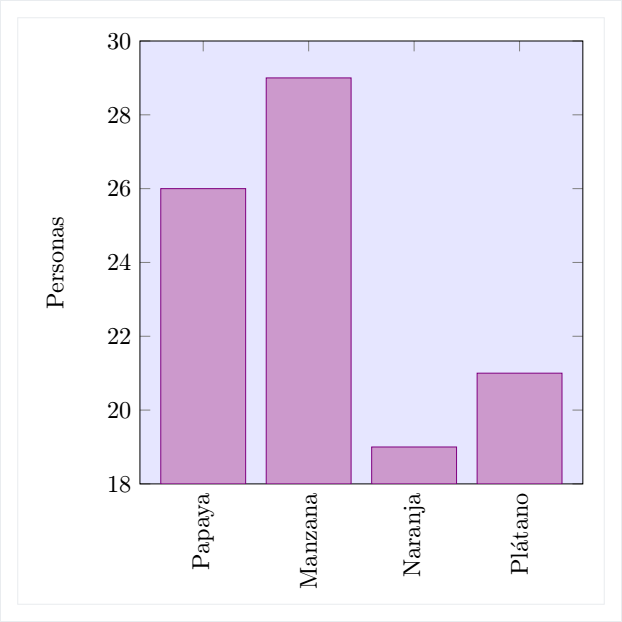
\includegraphics[width=\linewidth]{../images/imagen_barras_frutas01.png}
			\end{parts}
		\end{multicols}

	}

	\questionboxed[2]{Los resultados de una encuesta se muestran en la siguiente gráfica de barras:

		\begin{multicols}{2}
			\begin{parts}\normalsize
				\part ¿Cuántas personas participaron en la encuesta? \fillin[70][1.5cm]
				\part  ¿Cuál es la fruta menos preferida por las personas? \fillin[papaya][1.5cm]
				\part  ¿Cuál es la fruta preferida por las personas? \fillin[plátano][1.5cm]
				\part ¿Cuántas personas prefieren a las \textit{manzanas}.\fillin[16][1.5cm]
				\part ¿Cuántas personas prefieren a los \textit{plátanos}.\fillin[21][1.5cm]
				\part ¿Cuántas personas prefieren a las \textit{naranjas}.\fillin[19][1.5cm]

				\columnbreak%

				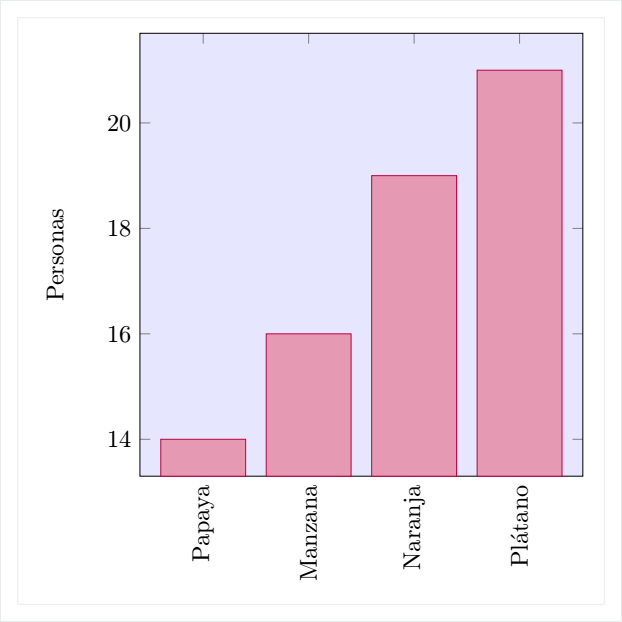
\includegraphics[width=\linewidth]{../images/imagen_barras_frutas02.png}
			\end{parts}
		\end{multicols}
	}


	% \subsection*{\ifprintanswers{Tablas de variación                }

	\questionboxed[2]{Contesta las siguientes preguntas:

		\begin{multicols}{2}
			\begin{parts}
				\part En la siguiente tabla se muestran la cantidad de personas que hay en aulas de una escuela. Si la cantidad de personas se mantienen constante, ¿cuántas personas habrá en 10 aulas?

				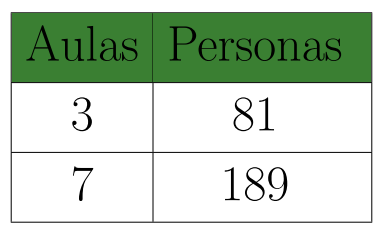
\includegraphics[width=0.45\linewidth]{../images/imagen_tabla_var06.png}
				\fillin[270][1.5cm]

				\part Con la información de la siguiente tabla, ¿cuál es el valor de x?

				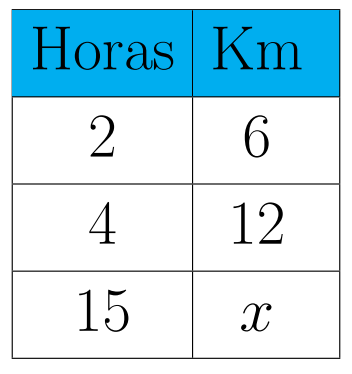
\includegraphics[width=0.35\linewidth]{../images/imagen_tabla_var03.png}
				\fillin[45][1.5cm]

				\part En la siguiente tabla se muestra el sueldo de una persona por hora trabajada. Si el pago se mantiene constante, ¿cuánto dinero recibe esta persona por hora trabajada?

				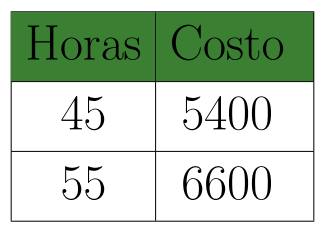
\includegraphics[width=0.4\linewidth]{../images/imagen_tabla_var05.png}
				\fillin[120][1.5cm]

				\part Con la información de la siguiente tabla, ¿cuál es el valor de x?

				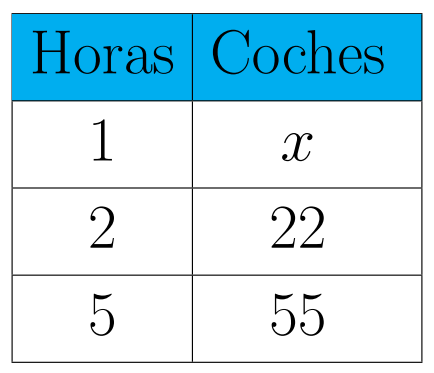
\includegraphics[width=0.42\linewidth]{../images/imagen_tabla_var04.png}
				\fillin[11][1.5cm]
			\end{parts}
		\end{multicols}
	}


	\addcontentsline{toc}{subsection}{Círculo}
	\subsection*{Círculo}
	% \subsection*{\ifprintanswers{Diámetro de un círculo             }
	% \subsection*{\ifprintanswers{Radio de un círculo                }
	\questionboxed[2]{Contesta las siguientes preguntas:

		\begin{multicols}{2}
			\begin{parts}
				\part ¿Cuál es el diámetro de un círculo que tiene un radio de 21.98?

				\begin{solutionbox}{1cm}
					\fillin[43.96][0cm]
				\end{solutionbox}

				\part ¿Cuál es el diámetro de un círculo que tiene un radio de 39.21?

				\begin{solutionbox}{1cm}
					\fillin[78.42][0cm]
				\end{solutionbox}

				\part ¿Cuál es el diámetro de un círculo que tiene un radio de 6.7?

				\begin{solutionbox}{1cm}
					\fillin[13.4][0cm]
				\end{solutionbox}

				\part ¿Cuál es el radio de un círculo que tiene un diámetro de 88.28?

				\begin{solutionbox}{1cm}
					\fillin[44.19][0cm]
				\end{solutionbox}

			\end{parts}
		\end{multicols}
	}

	% \subsection*{\ifprintanswers{Perímetro de un círculo            }
	% \subsection*{\ifprintanswers{Área de un círculo                 }

	\questionboxed[2]{Calcula el perímetro y área de los siguientes círculos:

		\begin{multicols}{3}
			\begin{parts}

				\part 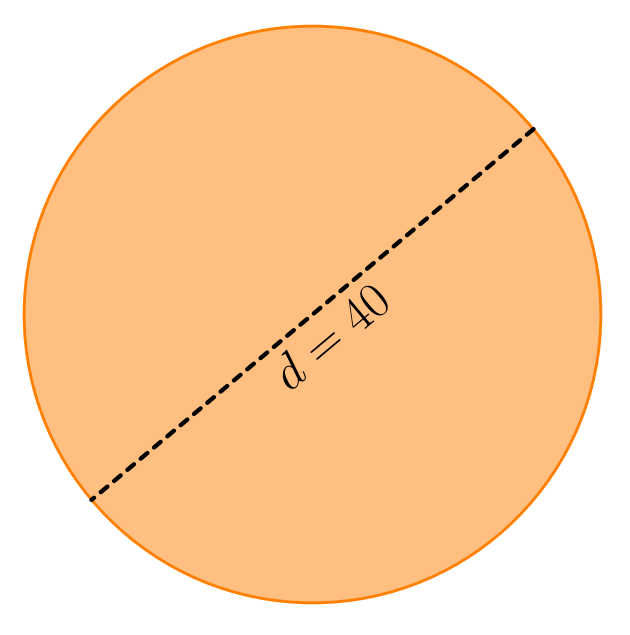
\includegraphics[width=0.8\linewidth]{../images/circulo01.png}\\
				\small Perímetro: \fillin[62.8][0.3in]  Área: \fillin[1256][0.3in]

				\begin{solutionbox}{1.2cm}\footnotesize
					% $P=8\pi=8(3.14)=25.12$ \\
					% $A=\pi(4)^2=3.14(4)^2=50.24$
				\end{solutionbox}

				\part 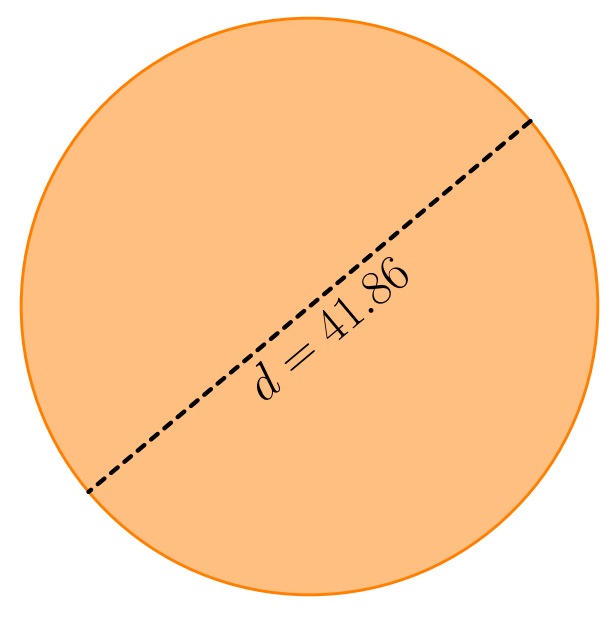
\includegraphics[width=0.8\linewidth]{../images/circulo02.png}\\
				\small Perímetro: \fillin[131.51][0.3in]  Área: \fillin[1376.22][0.3in]

				\begin{solutionbox}{1.2cm}\footnotesize
					% $P=2\pi r=2(3.14)(9.3)=58.4$ \\
					% $A=\pi r^2=3.14(9.3)^2=271.57$
				\end{solutionbox}

				\part 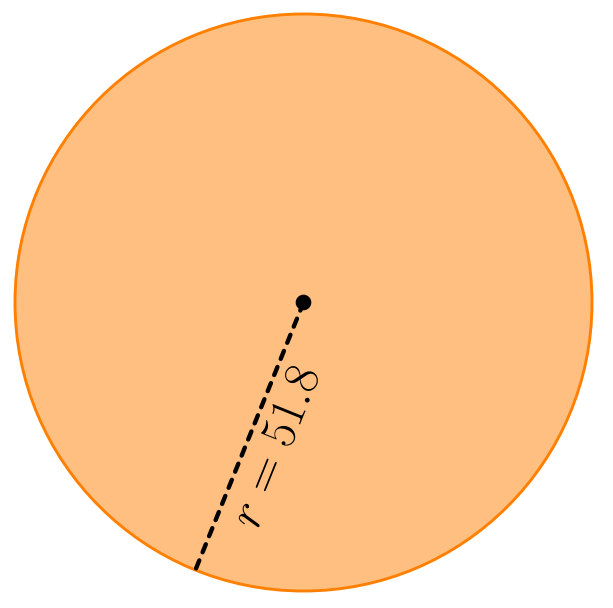
\includegraphics[width=0.8\linewidth]{../images/circulo03.png}\\
				\small Perímetro: \fillin[325.47][0.3in]  Área: \fillin[8429.65][0.3in]

				\begin{solutionbox}{1.2cm}\footnotesize
					% $P=2\pi r=2(3.14)(12)=75.36$ \\
					% $A=\pi r^2=3.14(12)^2=452.16$
				\end{solutionbox}

				\part 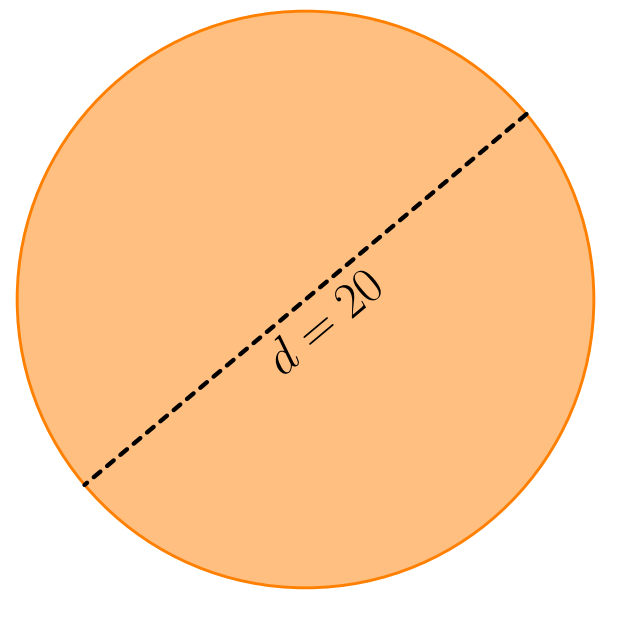
\includegraphics[width=0.8\linewidth]{../images/circulo04.png}\\
				\small Perímetro: \fillin[62.8][0.3in]  Área: \fillin[314][0.3in]

				\begin{solutionbox}{1.2cm}\footnotesize
					% $P=8\pi=8(3.14)=25.12$ \\
					% $A=\pi(4)^2=3.14(4)^2=50.24$
				\end{solutionbox}

				\part 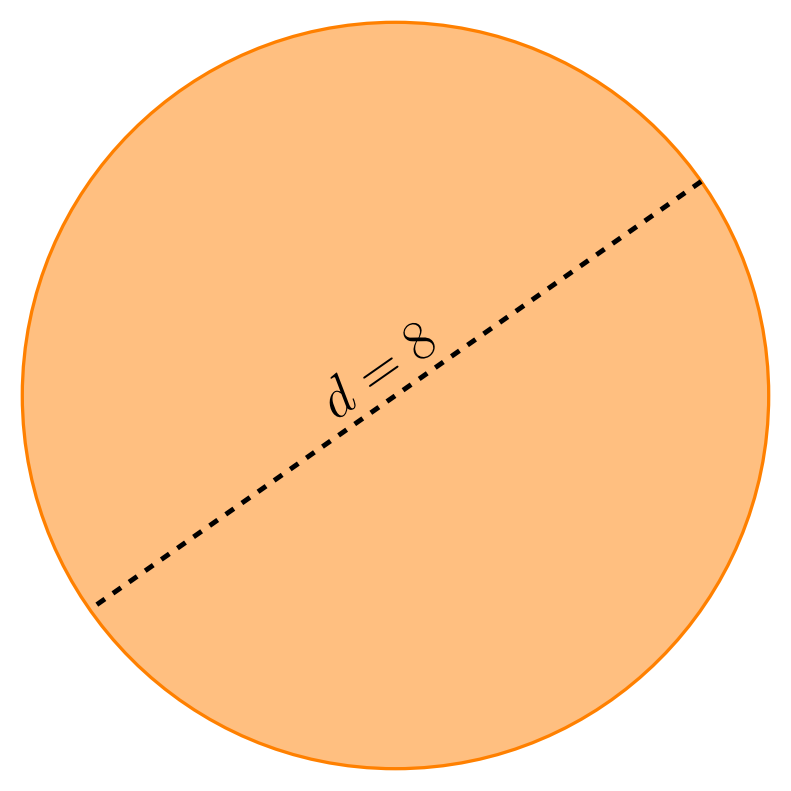
\includegraphics[width=0.8\linewidth]{../images/circulo05.png}\\
				\small Perímetro: \fillin[25.12][0.3in]  Área: \fillin[50.24][0.3in]

				\begin{solutionbox}{1.2cm}\footnotesize
					% $P=2\pi r=2(3.14)(9.3)=58.4$ \\
					% $A=\pi r^2=3.14(9.3)^2=271.57$
				\end{solutionbox}

				\part 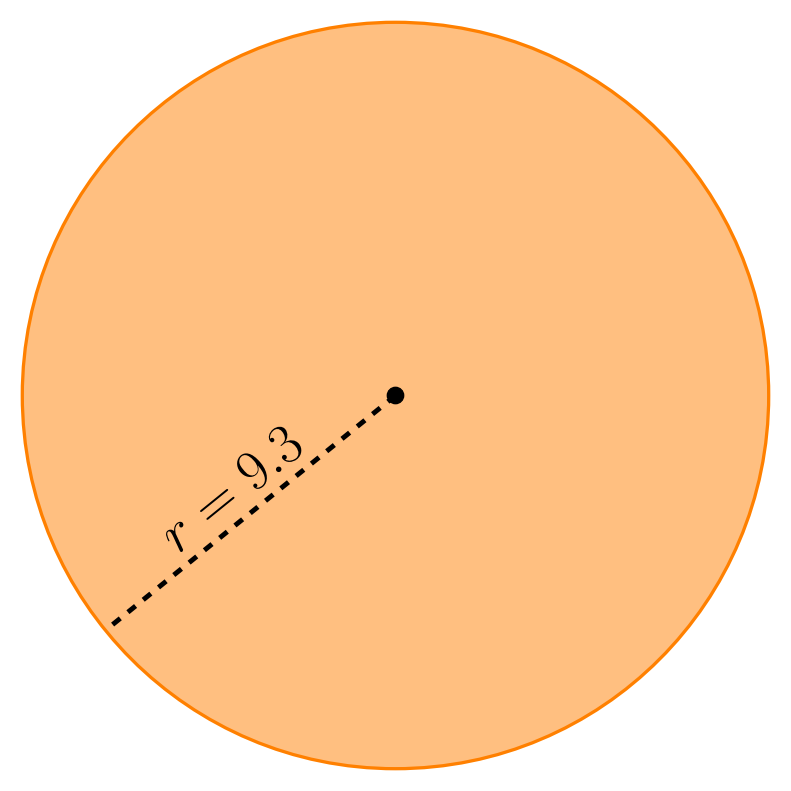
\includegraphics[width=0.8\linewidth]{../images/circulo06.png}\\
				\small Perímetro: \fillin[58.404][0.3in] Área: \fillin[271.57][0.3in]

				\begin{solutionbox}{1.2cm}\footnotesize
					% $P=2\pi r=2(3.14)(12)=75.36$ \\
					% $A=\pi r^2=3.14(12)^2=452.16$
				\end{solutionbox}
			\end{parts}
		\end{multicols}
	}





	% \subsection*{\ifprintanswers{Líneas del círculo                 }
	\addcontentsline{toc}{subsection}{Figuras geométricas}
	\subsection*{Figuras geométricas}

	% \subsection*{\ifprintanswers{Nombre de figuras                  }
	\questionboxed[2]{Escribe sobre la línea el nombre que recibe cada figura geométrica de acuerdo con su número de lados:

		\begin{multicols}{3}
			\begin{parts}
				\part 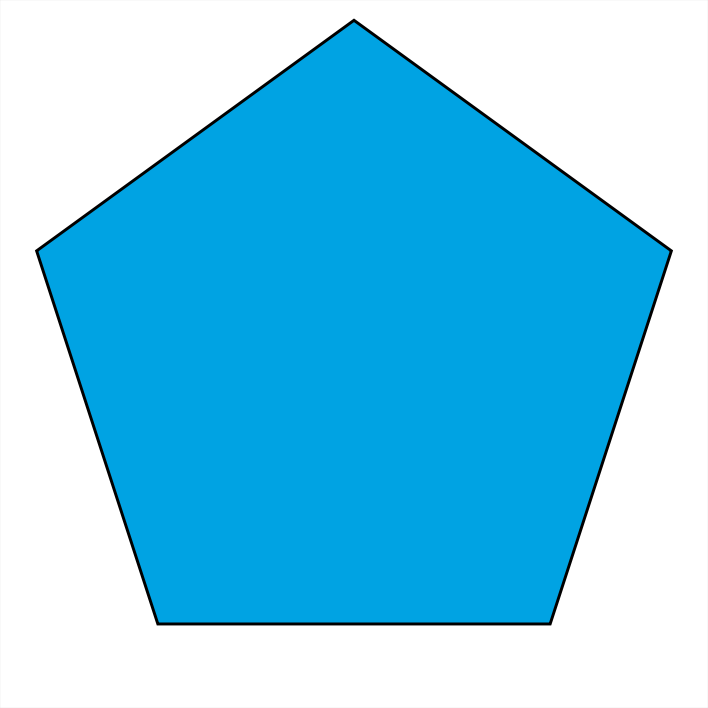
\includegraphics[width=75px]{../images/pentagono_azul.png}  \fillin[pentágono][0.75in]
				\part 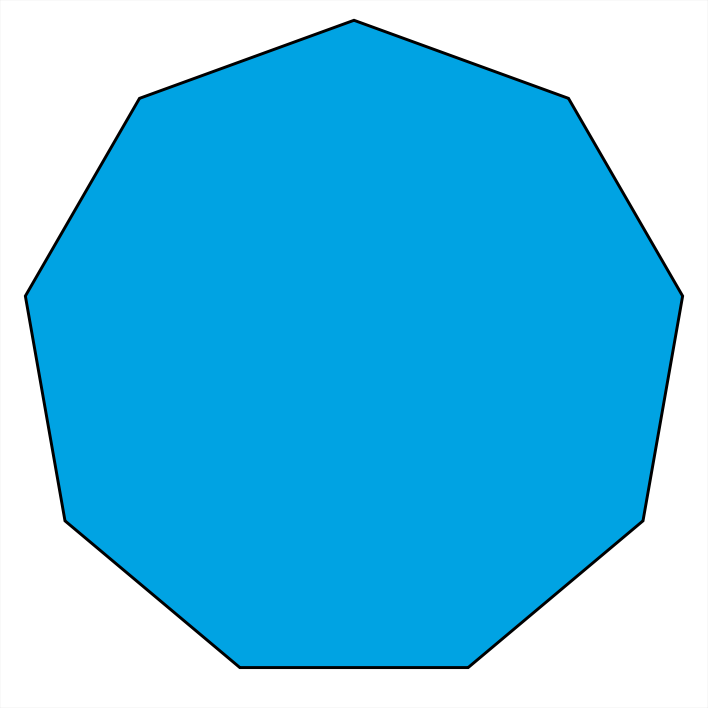
\includegraphics[width=75px]{../images/nonagono_azul.png}   \fillin[nonágono][0.75in]
				\part 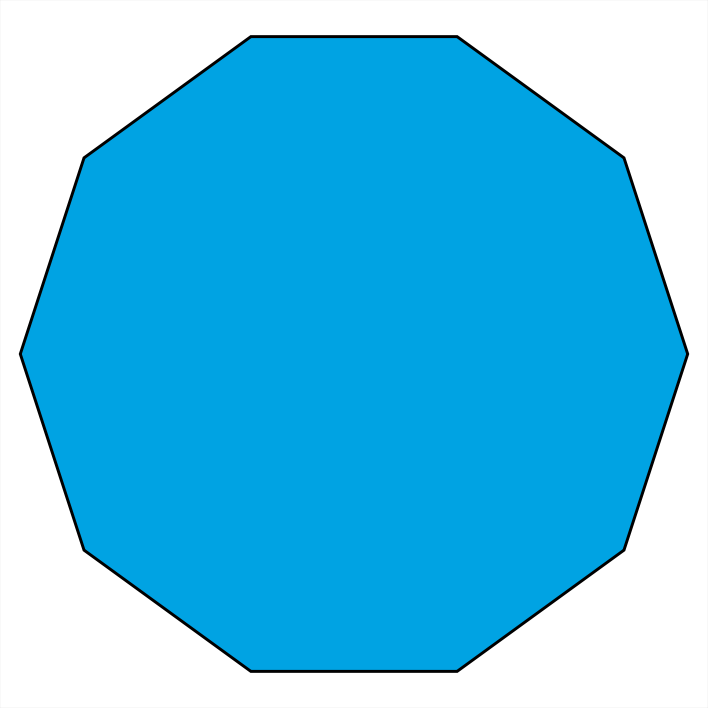
\includegraphics[width=75px]{../images/decagono_azul.png}   \fillin[decágono][0.75in]
				\part 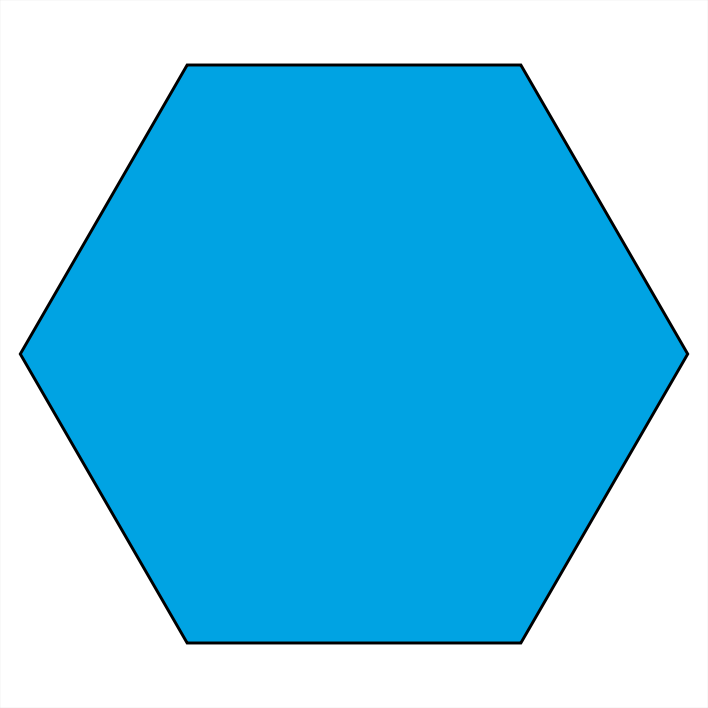
\includegraphics[width=75px]{../images/hexagono_azul.png}   \fillin[hexágono][0.75in]
				\part 
\includegraphics[width=75px]{../images/rectangulo_azul.png} \fillin[rectángulo][0.75in]
				\part 
\includegraphics[width=75px]{../images/cuadrado_azul.png}   \fillin[cuadrado][0.75in]
			\end{parts}
		\end{multicols}
	}


	% \subsection*{\ifprintanswers{Elementos de figuras               }
	% \subsection*{\ifprintanswers{Perímetro  }
	\questionboxed[4]{Contesta las preguntas sobre perímetros de figuras geométricas

		\begin{multicols}{2}
			\begin{parts}
				\part ¿Cuál es el perímetro de un rectángulo cuya base mide 38 y su altura mide 19?

				\begin{solutionbox}{1cm}
					\[P=38+19+38+19=\color{red}114\]
				\end{solutionbox}

				\part ¿Cuál es el perímetro de un cuadrado que sus lados miden 5?

				\begin{solutionbox}{1cm}
					\[P=5+5+5+5=\color{red}20\]
				\end{solutionbox}

				\part ¿Cuál es el perímetro de un pentágono que sus lados miden 18?

				\begin{solutionbox}{1cm}
					\[P=18 \times 5=\color{red}90\]
				\end{solutionbox}

				% \part ¿Cuál es el perímetro de un octágono que sus lados miden 15?

				% \begin{solutionbox}{1cm}
				% 	\[P=15 \times 8=\color{red}120\]
				% \end{solutionbox}

				\part ¿Cuál es el perímetro de un rombo que sus lados miden 16?

				\begin{solutionbox}{1cm}
					\[P=16 \times 4=\color{red}64\]
				\end{solutionbox}

			\end{parts}
		\end{multicols}
	}

	% \subsection*{\ifprintanswers{Área       }
	\questionboxed[2]{Contesta las preguntas sobre áreas de figuras geométricas

		\begin{multicols}{2}
			\begin{parts}
				\part ¿Cuál es el área de un triángulo cuya base mide 18 y su altura mide 11?

				\begin{solutionbox}{1.5cm}
					\[A=\dfrac{18 \times 11}{2}=\color{red}99\]
				\end{solutionbox}


				\part ¿Cuál es el área de un cuadrado que sus lados miden 29?

				\begin{solutionbox}{1.5cm}
					\[A=29 \times 29=\color{red}841\]
				\end{solutionbox}

			\end{parts}
		\end{multicols}
	}

	% \subsection*{\ifprintanswers{Resolución de problemas            }
	\addcontentsline{toc}{subsection}{Resolución de problemas}
	\subsection*{Resolución de problemas}
	% \subsection*{\ifprintanswers{Unidades de tiempo y reloj         }

	\questionboxed[2]{
		\begin{multicols}{2}
			\begin{parts}
				\part Convierte 23 horas a minutos:    \begin{solutionbox}{1cm}\fillin[1380][0in]\end{solutionbox}
				\part Convierte 27 horas a segundos:   \begin{solutionbox}{1cm}\fillin[97200][0in]\end{solutionbox}
				\part Convierte 3.9 horas a minutos:   \begin{solutionbox}{1cm}\fillin[234][0in]\end{solutionbox}
				\part Convierte 4.8 minutos a segundos:\begin{solutionbox}{1cm}\fillin[288][0in]\end{solutionbox}
			\end{parts}
		\end{multicols}
	}

	% \subsection*{\ifprintanswers{Cuerpos geométricos 1              }
	% \subsection*{\ifprintanswers{Cuerpos geométricos 2              }
	% \subsection*{\ifprintanswers{Resolución de problemas 1          }
	% \subsection*{\ifprintanswers{Resolución de problemas 2          }

	\questionboxed[2]{Resuelve los siguientes problemas:

		\begin{multicols}{2}
			\begin{parts}
				\part Alejandro quiere poner una barda alrededor de un terreno cuadrangular que mide 22 metros por lado. ¿Cuánta barda necesitará Alejandro para poner barda en todo el terreno?

				\begin{solutionbox}{1cm}
					\fillin[88][0in]
				\end{solutionbox}

				\part Para darle mantenimiento a una alberca olímpica se pone cinta alrededor de esta. Si la alberca tiene 50 metros de largo y 25 metros de ancho, ¿cuánta cinta se necesita para darle la vuelta a la alberca?

				\begin{solutionbox}{1cm}
					\fillin[150][0in]
				\end{solutionbox}


				\part Bruno corre todos los días en un parque de forma rectangular el cual mide 75 metros de largo y 40 metros de ancho. ¿Cuántos metros corre Bruno por una vuelta?

				\begin{solutionbox}{1cm}
					\fillin[230][0in]
				\end{solutionbox}

				\part Bruno corre todos los días en un parque de forma rectangular el cual mide 50 metros de largo y 28 metros de ancho. Si al día le da 4 vueltas al parque, ¿cuántos metros habrá corrido en total Bruno?

				\begin{solutionbox}{1cm}
					\fillin[624][0in]
				\end{solutionbox}
			\end{parts}
		\end{multicols}
	}

	\addcontentsline{toc}{subsection}{Sistema de unidades}
	\subsection*{Sistema de unidades}
	% \subsection*{\ifprintanswers{Multiplicaciones por múltiplos de 10}
	% \subsection*{\ifprintanswers{Divisiones por múltiplos de 10     }
	% \subsection*{\ifprintanswers{Unidades de longitud               }
	% \subsection*{\ifprintanswers{Unidades de masa                   }
	% \subsection*{\ifprintanswers{Unidades de capacidad              }
	\questionboxed[2]{Realiza las siguientes operaciones:

		\begin{multicols}{2}
			\begin{parts}
				% \part $ 93.2 \times 1000=$   \fillin[93200][0.5in]
				\part $ 84.2 \times 100=$   \fillin[8420][0.5in]
				\part $ 66.472 \times 10000=$   \fillin[664720][0.5in]
				\part $ 192.3 \times 10=$   \fillin[1923][0.5in]
				\part $ 26.9 \times 1000=$   \fillin[26900][0.5in]
				\part $ 81.674 \times 100000=$   \fillin[8167400][0.5in]
				\part $ 1.2 \times 1000=$   \fillin[1200][0.5in]
				\part $ 7.8 \times 10=$   \fillin[78][0.5in]
				\part $ 38093 \divisionsymbol 10=$   \fillin[3809.3][0.5in]
				\part $ 28 \divisionsymbol 1000=$   \fillin[0.028][0.5in]
				\part $ 44567 \divisionsymbol 100=$   \fillin[445.67][0.5in]
				\part $ 678 \divisionsymbol 1000=$   \fillin[0.678][0.5in]
				\part $ 7.1 \divisionsymbol 10=$   \fillin[0.71][0.5in]
				\part $ 51 \divisionsymbol 100=$   \fillin[0.51][0.5in]
				\part $ 3.9 \divisionsymbol 100=$   \fillin[0.039][0.5in]
				% \part $ 2.4 \divisionsymbol 100=$   \fillin[0.024][0.5in]
				% \part $ 34 \divisionsymbol 10=$   \fillin[3.4][0.5in]
				% \part $ 6.3 \divisionsymbol 10000=$   \fillin[0.00063][0.5in]
			\end{parts}
		\end{multicols}
	}




	\questionboxed[4]{Realiza las siguientes conversiones de unidades de longitud y masa:

		\begin{multicols}{2}
			\begin{parts}\normalsize
				\part De 157 kilómetros a hectómetros. \hfill \fillin[1570][0.6in] hm
				\part De 25 centímetros a milímetros.  \hfill \fillin[250][0.6in] mm
				\part De 27 kilómetros a decámetros.   \hfill \fillin[2700][0.6in] Dm
				\part De 17 kilómetros a hectómetros.  \hfill \fillin[170][0.6in] hm
				\part De 69 kilómetros a centímetros.  \hfill \fillin[6900000][0.6in] cm
				\part De 59 decímetros a centímetros.  \hfill \fillin[590][0.6in] cm
				\part De 26 metros a decímetros.       \hfill \fillin[260][0.6in] dm
				\part De 4 kilómetros a milímetros.    \hfill \fillin[4000000][0.6in] mm
				\part De 135 kilómetros a decámetros.  \hfill \fillin[13500][0.6in] Dm
				\part De 112 kilómetros a hectómetros. \hfill \fillin[1120][0.6in] hm
				\part De 205 gramos a decigramos    \hfill \fillin[2050][0.5in] dg
				\part De 25 kilogramos a gramos     \hfill \fillin[25000][0.5in] g
				\part De 58 kilogramos a gramos     \hfill \fillin[58000][0.5in] g
				\part De 45 decagramos a gramos     \hfill \fillin[450][0.5in] g
				\part De 134 gramos a decigramos    \hfill \fillin[1340][0.5in] dg
				\part De 282 gramos a miligramos    \hfill \fillin[282000][0.5in] mg
				\part De 117 decagramos a gramos    \hfill \fillin[1170][0.5in] g
				\part De 17 decigramos a miligramos \hfill \fillin[1700][0.5in] mg
				\part De 115 gramos a centigramos   \hfill \fillin[11500][0.5in] cg
				\part De 62 gramos a miligramos     \hfill \fillin[62000][0.5in] mg
			\end{parts}
		\end{multicols}
	}


	
\end{questions}
\end{document}